\chapter{Estado del arte}

En este apartado lo que pretende es mostrar como se encuentra el panorama en el cual vamos a llevar
acabo este proyecto. Para ello, en primer lugar voy a analizar las soluciones parecidas ya existentes,
donde se presentarán las principales alternativas a nuestra idea de proyecto, de forma que analicemos
los requisitos de nuestro sistema comparándolo con los de aquellos que ya existen.

\section{Análisis de mercado}

Como he comentado ya con anterioridad, el acceso a los datos sobre las defunciones es de dominio público
y por tanto accesible por cualquiera. Dado que este proyecto se centra en la obtención y tratamiento de
estos datos. Es importante conocer si existen ya aplicaciones que presten funcionalidades parecidas a las que
quiero implementar.

\subsection{Instituto Nacional de Estadística}
Podemos ver la página del \cite{INE} Instituto Nacional de Estadística que es un referente a la hora de obtener
y mostrar datos, además existen repositorios de datos de interés para este trabajo.
Vamos a utilizar los datos publicados sobre defunciones según causa de muerte para investigar la interfaz que nos
proponen desde el instituto. Voy a detallas las funcionalidades que he encontrado que creo que he de tener
en cuanta para mejorar.
\begin{itemize}
    \item La vista de la página puede ser algo compleja para algunos usuarios.
    \item No es totalmente responsive.
    \item Cuando seleccionas las variables y queremos obtener dicha visualización de datos, la página se
    recarga y nos muestra otra página donde no tenemos a mano las variables para realizar
    otra consulta instantáneamente.
    \item No tenemos visualización gráfica. Te redirige a descargar el programa PC-Axis únicamente disponible para
    Windows si quieres ver mas detalles sobre los datos almacenados.
\end{itemize}

\begin{figure}[]
	\centering
	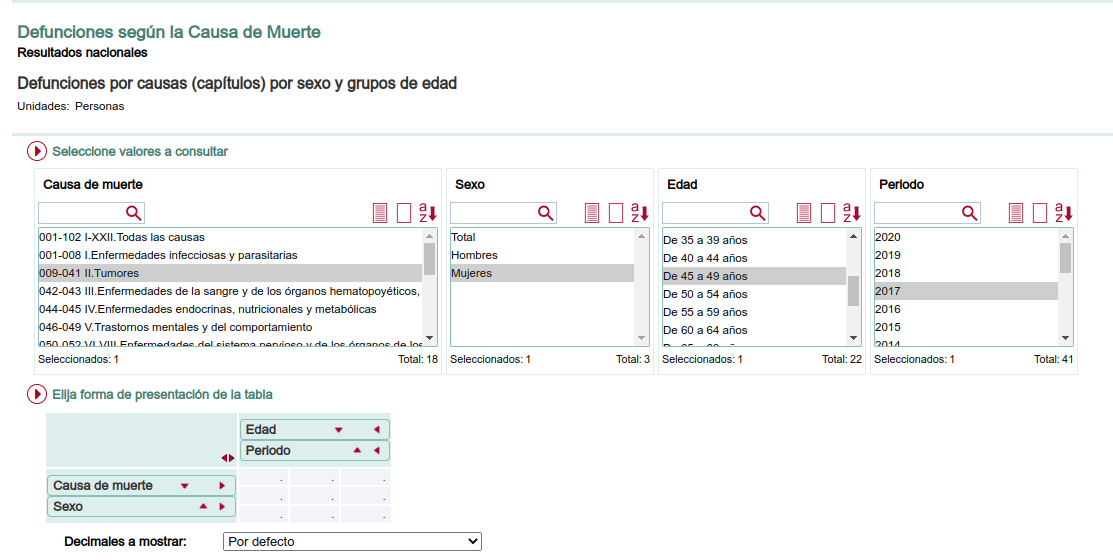
\includegraphics[scale=0.5]{doc/logos/imgs/ine1.png}
	\caption{ \cite{INE}  Vista principal para obtener datos en el INE }
    \label{fig:worst_f_value}
\end{figure}

\begin{figure}[]
	\centering
	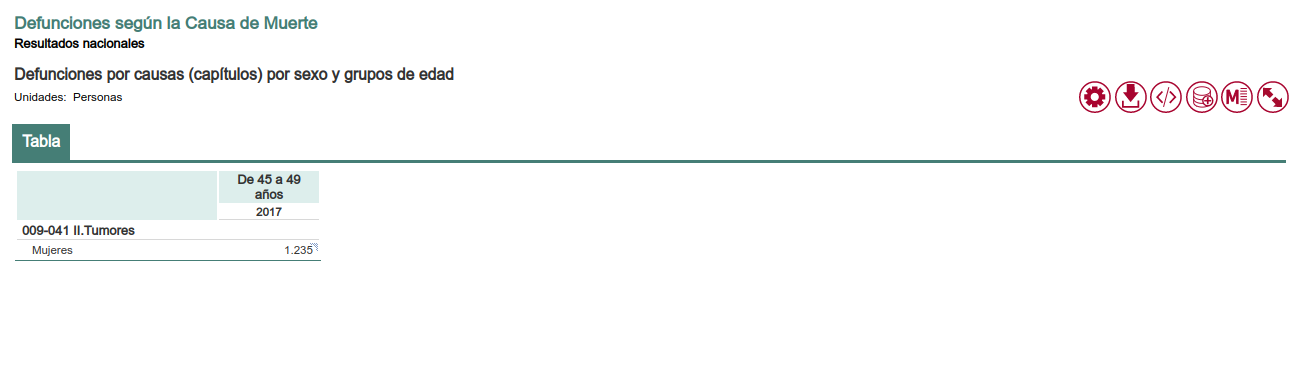
\includegraphics[scale=0.5]{doc/logos/imgs/ine2.png}
	\caption{ \cite{INE} Vista resultado cuando se han filtrado los datos a obtener }
    \label{fig:worst_f_value}
\end{figure}
Por otro lado no podemos perder de vista, la integridad con la que ofrece los datos, los distintos formatos
de descarga que nos ofrece y las notas explicativas sobre como se ha procedido a la obtención de los mismos.

\subsection{Instituto de Salud Carlos III}
En la página del Instituto de Salud Carlos III \cite{isciii} podemos encontrar muchas entradas hablando sobre
la mortalidad de la población y morbilidad apoyada de \cite{momo} gráficas MoMo que son gráficas de desviaciones de mortalidad
diaria respecto a la esperada según las series históricas de mortalidad, estas constituyen un sistema de vigilancia
que proporciona información sobre el impacto en mortalidad de la población. Estas son entregables en formato web y PDF.

A pesar de la valiosísima información que estos informes pueden arrojar no es lo que persigue este trabajo que se
centra en la obtención de datos crudos. El instituto pone a disposición de los ciudadanos tres servidores interactivos.

\subsubsection{Servidor Arïadna}
Nos permite consultar información sobre las causas de defunción atendiendo a cuatro variables:
\begin{enumerate}
  \item Indicador.
  \item Causa.
  \item Período, años.
  \item Sexo.
  \item Comunidad Autónoma.
  \item Provincia.
\end{enumerate}

Los indicadores pueden ser:
\begin{enumerate}
  \item Tasa ajustada a la población europea.
  \item Tasa ajustada a la población mundial.
  \item Tasa truncada: tasa ajustada de mortalidad limitada a los 35-64 años de edad.
  \item Índice comparativo de mortalidad: Es el cociente entre la tasa ajustada por edad en cada provincia y la tasa
  ajustada para el conjunto de España.
  \item Tasa cruda: la tasa cruda de mortalidad es la proporción de personas que fallecen con respecto al total
  de la población en un período determinado. Se expresa habitualmente como el número de defunciones al año
  por cada 100.000 personas.
  \item Número de defunciones
\end{enumerate}

\begin{figure}[]
	\centering
	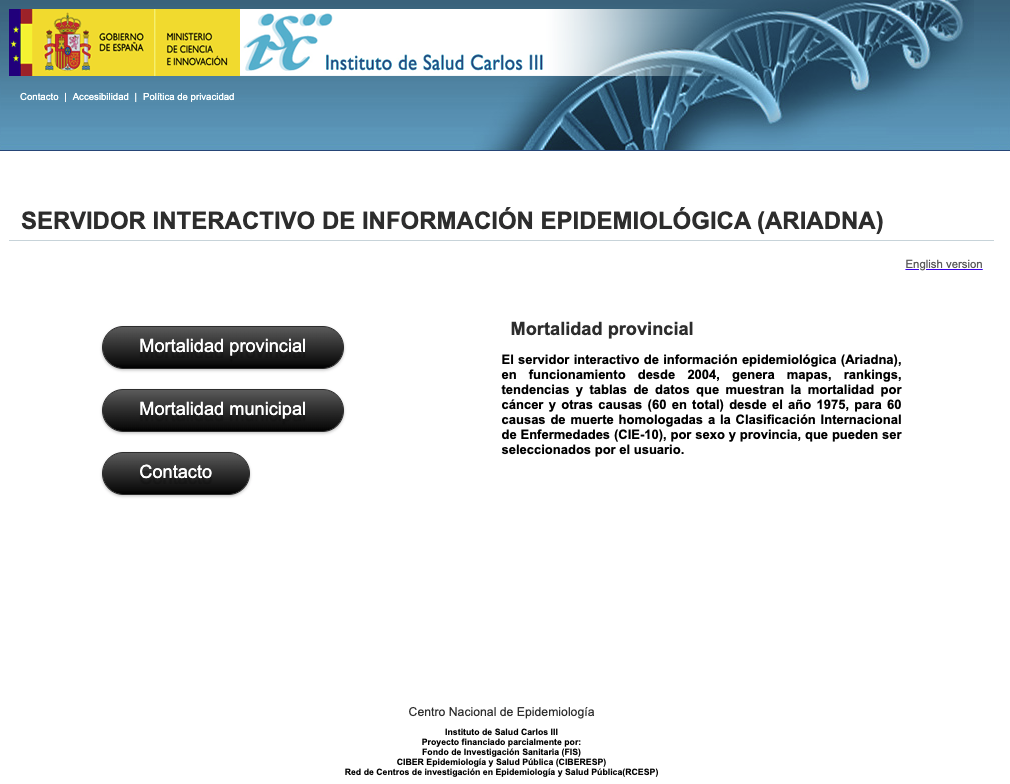
\includegraphics[scale=0.5]{doc/logos/imgs/ariadna1.png}
	\caption{ \cite{ariadna} Vista principal del servidor Arïadna }
    \label{fig:worst_f_value}
\end{figure}

\begin{figure}[]
	\centering
	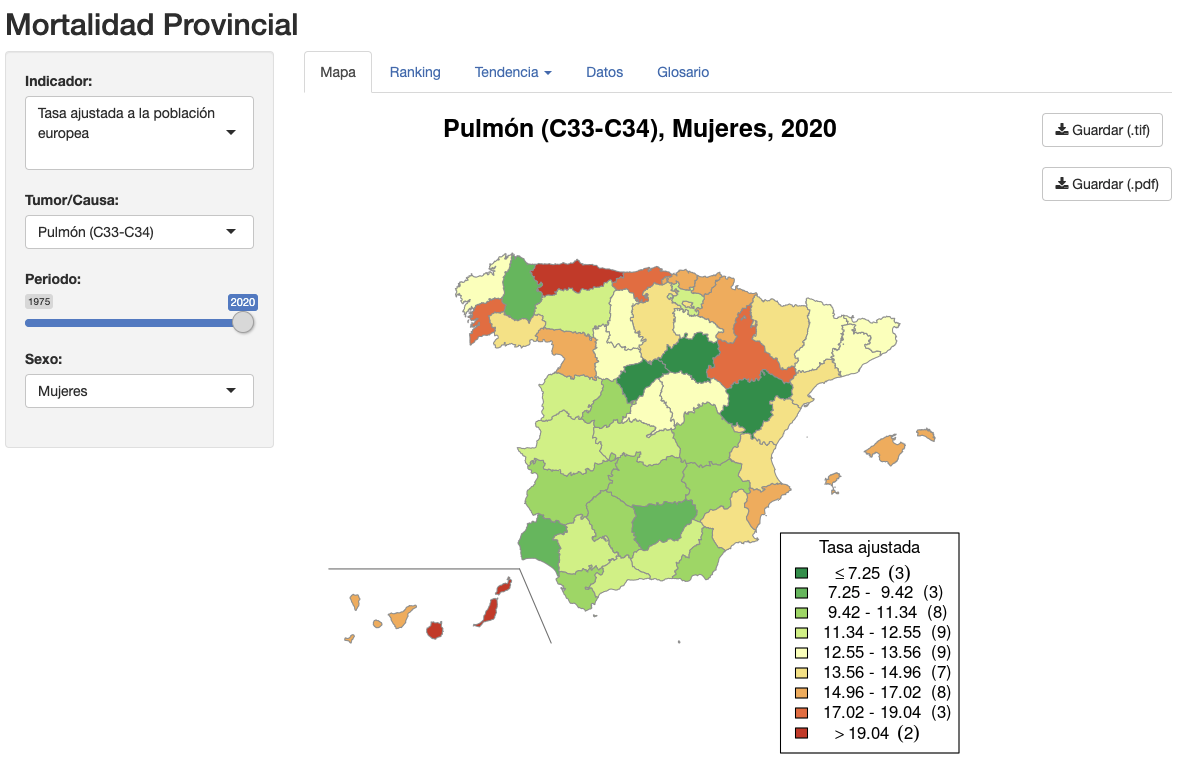
\includegraphics[scale=0.5]{doc/logos/imgs/ariadna2.png}
	\caption{ \cite{ariadna} Vista por mortalidad provincial }
    \label{fig:worst_f_value}
\end{figure}

Los datos son ofrecidos mediante un mapa de España interactivo podemos observar también gráficas de todas las
provincias y la media nacional así como una tabla con los datos. Esta página permite descargarse los datos pero
únicamente en formato CSV y sólo de 10 tuplas en 10 tuplas sobre las variables filtradas. Lo que hizo que me pusiera en 
contacto con el ISCIII si quería tener estos datos para trabajar.

\subsubsection{Servidor Raziël}
Es un servidor interactivo genera mapas y gráficas de España por comunidades autónomas, y tablas de datos que muestran 
las diferencias en la mortalidad por diversas causas, desde el año 1980, de acuerdo con los criterios que de el usuario.
Nos permite consultar información sobre las causas de defunción atendiendo a cuatro variables:
\begin{enumerate}
    \item Indicador.
    \item Causa.
    \item Período, años.
    \item Sexo.
    \item Grupo de edades.
    \item Comunidad Autónoma.
  \end{enumerate}


\section{Mi propuesta ante el estado del arte}
Sin perder de vista los objetivos y usuarios diana a utilizar este trabajo, contrastar las idea
que tenía con las existentes ha sido muy útil. Para mejorar la accesibilidad de estos datos con las soluciones implementadas 
ya por los organismos citados anteriormente he recogido someramente los siguientes puntos en los que ha de guiarse la 
solución. Las principales deficiencias encontradas y objetivo a subsanar son:
\begin{itemize}
    \item Inexistencia de una API para que programadores y usuarios externos puedan obtener los datos
    de forma uniforma y utilizando protocolos actuales.
    \item La información es exportada en ficheros demasiados grandes y pesados para trabajar con ellos.
    \item Aplicaciones basadas en el modelo C/S que a cada cambio hace que se recarguen las páginas y pierdas
    la instantaneidad tan cómoda para consultar como varían los datos
\end{itemize}

De otra manera, si queremos consultar datos acerca de las provincias es necesario cambiarse de banco de datos o si quieres
consultar las enfermdades clasificadas según CIE-10 con los grupos de edad es imposible pues estas informaciones
se encuentran en servicios distintos. Voy a intentar unificar estas dos fuentes de forma que podamos obtener esta información
desde un mismo servicio.
